\section{Problem no.2}

\subsection{Simulation with \textit{Design Studio}}

In order to verify and optimize the design of the BFN we decided to use \textit{CST Design Studio}, one of the various tools offered by \textit{CST Studio Suite}, which allows the user to design a microstrip network via schematic, to optimize it through the embedded optimization tool and then to create a layout of the whole project that can easily be exported in \textit{CST Microwave Studio} for further simulations.

\par\medskip
\noindent
Figure \ref{BFN_schematic} shows how a schematic looks like in \textit{CST Design Studio}. The isolated block is needed in order to assign to the structure fundamental properties such as thickness of the ground plane and dielectric constant of the substrate, while the other blocks build up the whole structure, allowing the creation of lines with assigned width and length and even bends (for example mitered) and junctions.

\begin{figure}[H]
\centering
\includegraphics[scale=0.4]{BFN_schematic.png}
\caption{BFN schematic on \textit{CST Design Studio}}
\label{BFN_schematic}
\end{figure}

\par\medskip
\noindent
As a first step the BFN has been drawn with the dimensions calculated during the design phase and then we specified that we wanted to see the S parameters at all ports (port 1 has an impedance of 50 $\Omega$, ports 2 to 5 have an impedance of 120 $\Omega$, since they take the place of the patches) as a simulation result. Next, the optimizer was set with the initial goal of tuning the S\textsubscript{11} parameter so to make it resonate at 2.45 GHz with the highest possible precision, obtaining the result shown in figure \ref{BFN_S11}.

\begin{figure}[H]
\centering
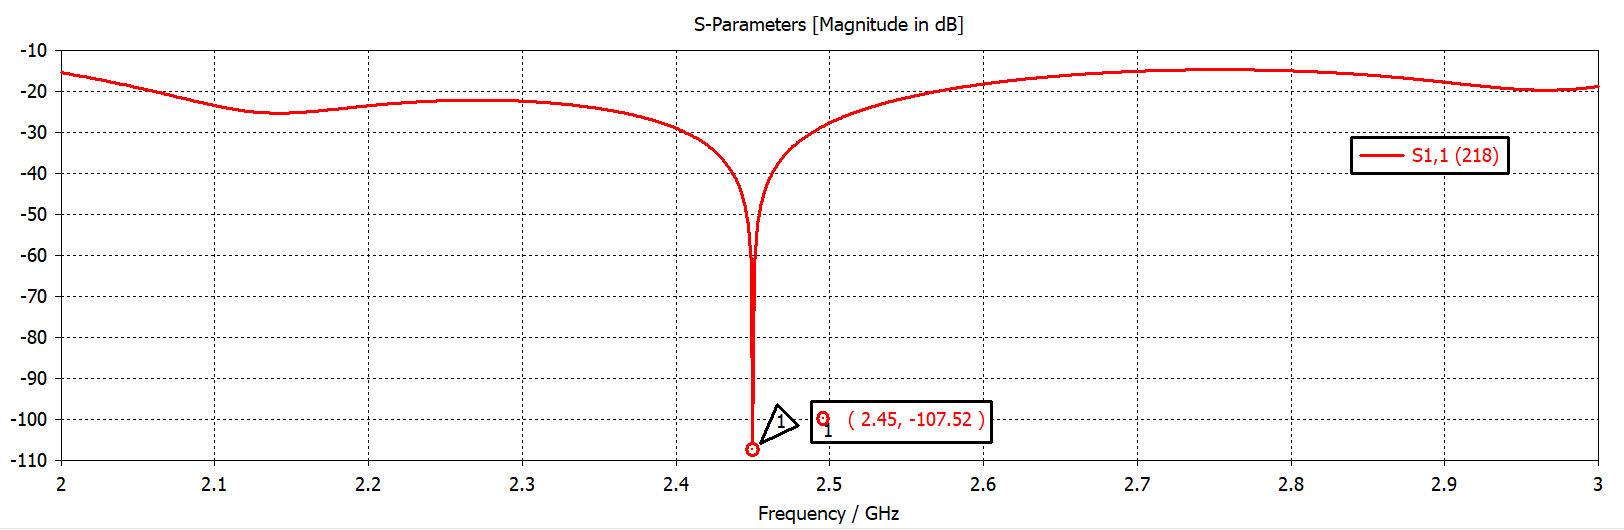
\includegraphics[scale=0.35]{BFN_S11.png}
\caption{S\textsubscript{11} parameter of our BFN}
\label{BFN_S11}
\end{figure}

\par\medskip
\noindent
As one can see, S\textsubscript{11} is pretty well shaped and furthermore the resonance at the desired frequency is strong and the obtained bandwidth is quite large.

\par\medskip
\noindent
Next step is the verification of the obtained tapering and phasing, which can be done by checking the value of the S\textsubscript{ij} parameters.

\begin{figure}[H]
\centering
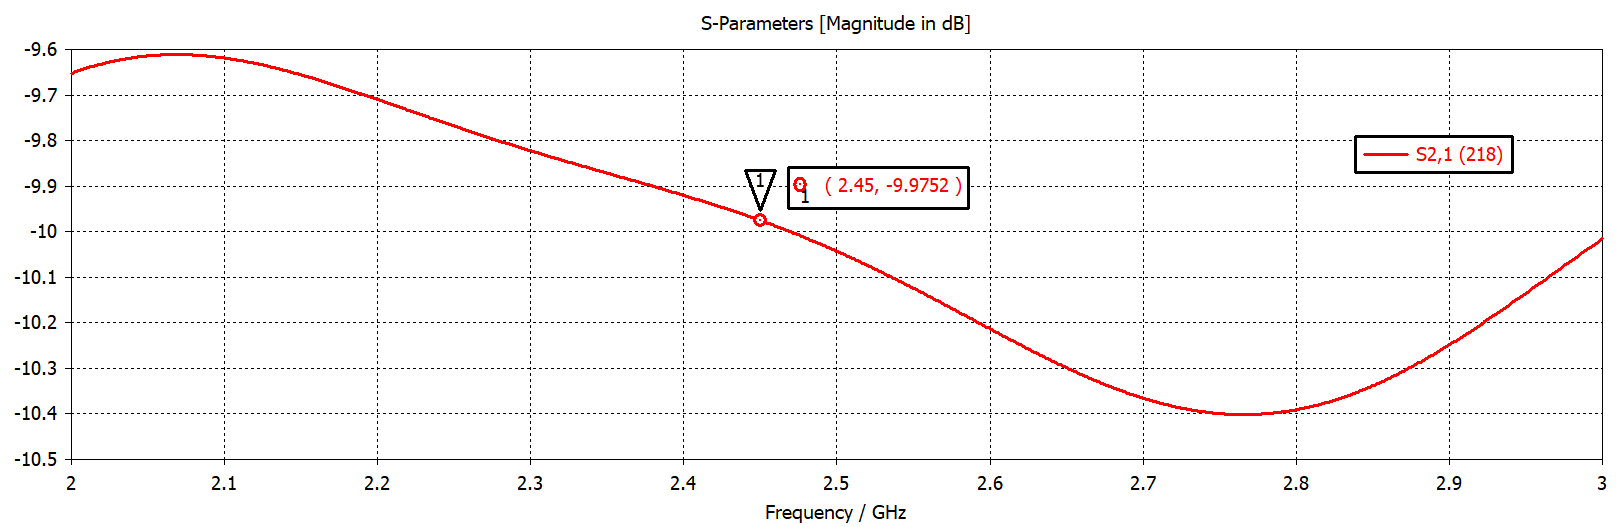
\includegraphics[scale=0.35]{S21Amp.png}
\caption{S\textsubscript{21} parameter of our BFN}
\label{S21Amp}
\end{figure}

\begin{figure}[H]
\centering
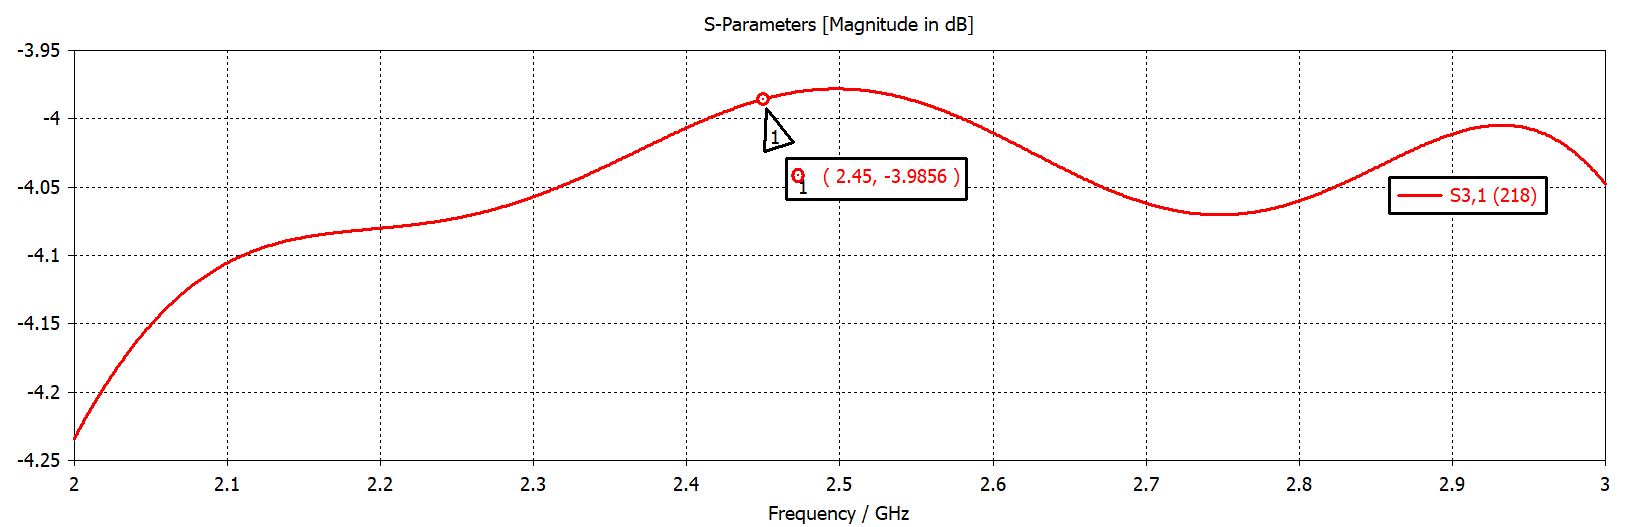
\includegraphics[scale=0.35]{S31Amp.png}
\caption{S\textsubscript{31} parameter of our BFN}
\label{S31Amp}
\end{figure}

\begin{figure}[H]
\centering
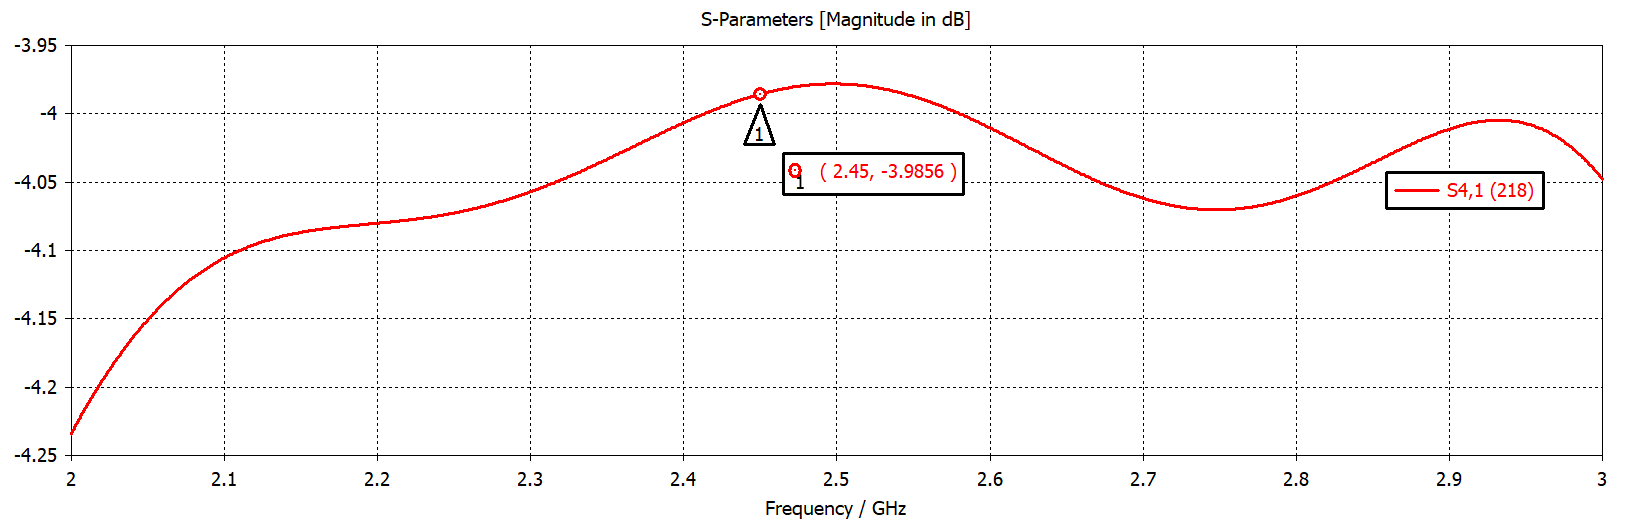
\includegraphics[scale=0.35]{S41Amp.png}
\caption{S\textsubscript{41} parameter of our BFN}
\label{S41Amp}
\end{figure}

\begin{figure}[H]
\centering
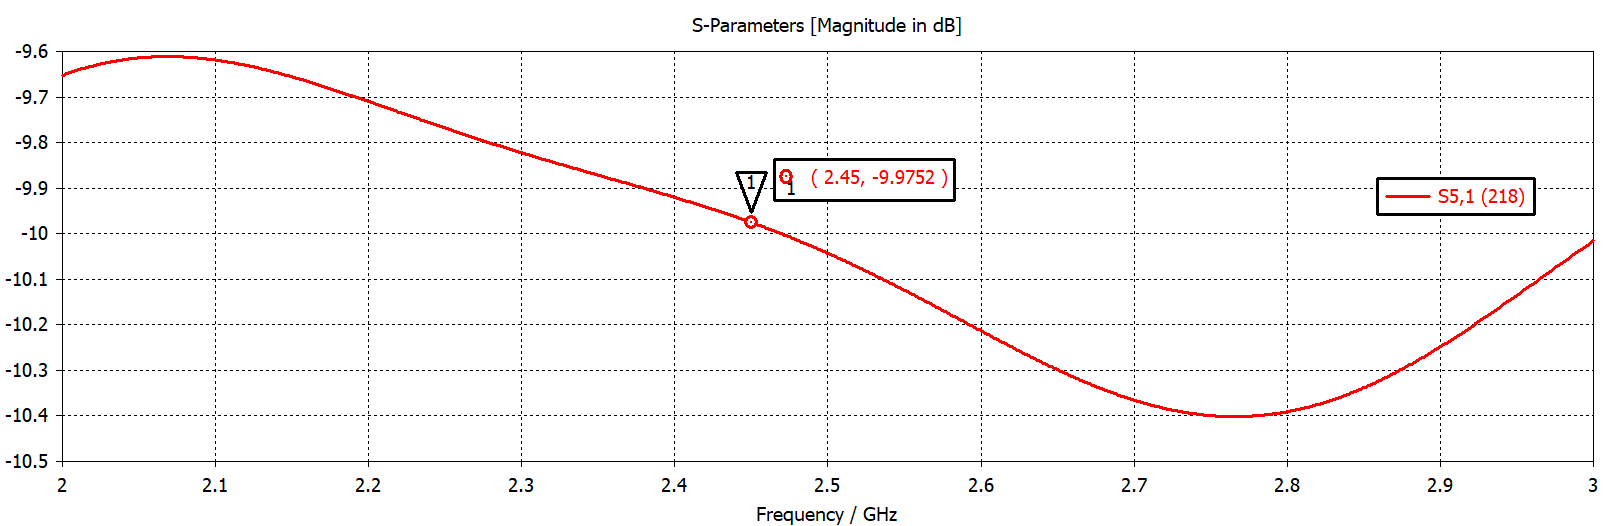
\includegraphics[scale=0.35]{S51Amp.png}
\caption{S\textsubscript{51} parameter of our BFN}
\label{S51Amp}
\end{figure}

\par\medskip
\noindent
The power ratio between the central elements of the array (ports 3 and 4) and the edge ones (ports 1 and 5) turns out to be 5.98 dB.

\par\medskip
\noindent
Last but not least, we have to verify that the phase shift between the output ports is as close as possible to 0.

\begin{figure}[H]
\centering
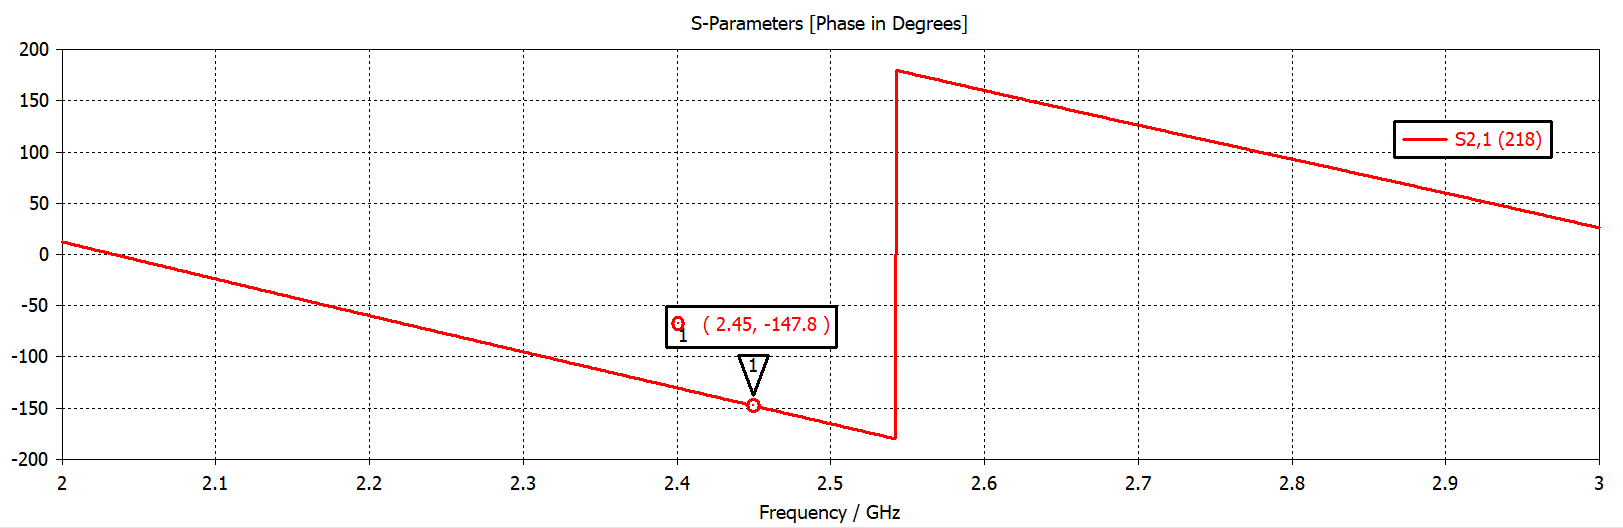
\includegraphics[scale=0.35]{S21p.png}
\caption{S\textsubscript{21} parameter (phase), coinciding with S\textsubscript{51}}
\label{S21phase}
\end{figure}

\begin{figure}[H]
\centering
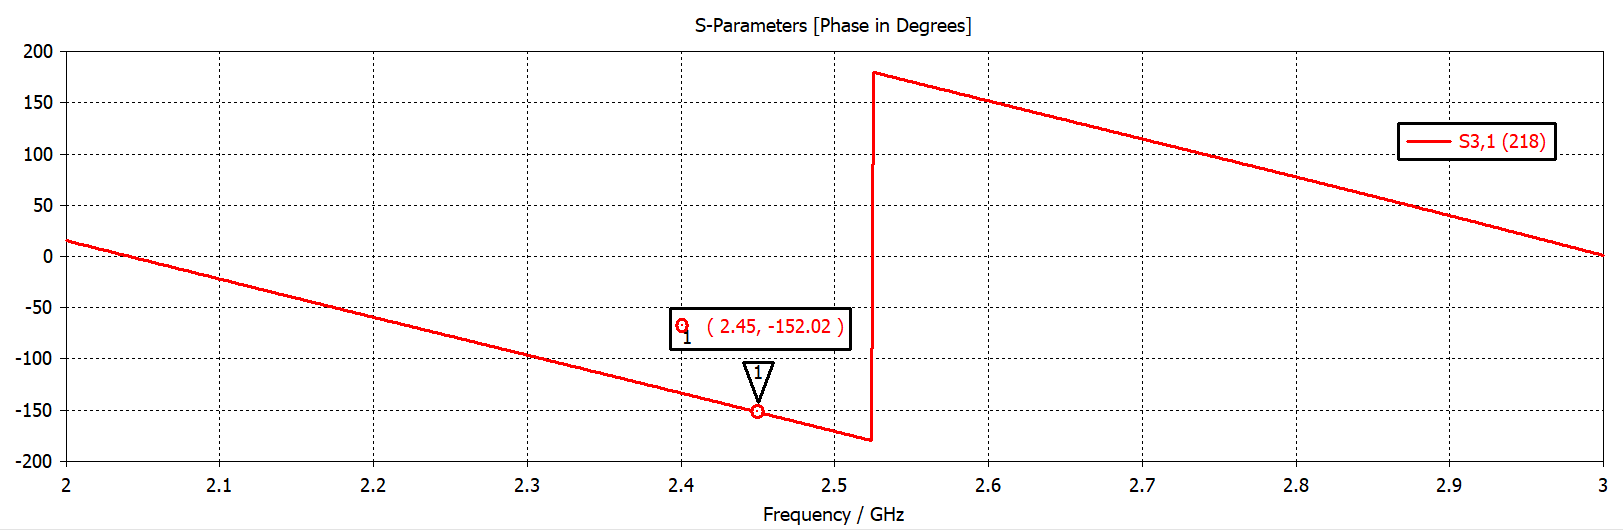
\includegraphics[scale=0.35]{S31p.png}
\caption{S\textsubscript{31} parameter (phase), coinciding with S\textsubscript{41}}
\label{S31phase}
\end{figure}

\par\medskip
\noindent
The phase difference between center and edge elements is around 4\textsuperscript{$\circ$}. A simulation of the complete structure in \textit{Microwave Studio} will tell us whether this lack of precision will affect the behavior of the array a lot or it will result either way to be broadside, as expected.

\par\medskip
\noindent
In order to have a visual impact of what the schematic is translated into in terms of layout, figure \ref{layout} shows the resulting structure.

\begin{figure}[H]
\centering
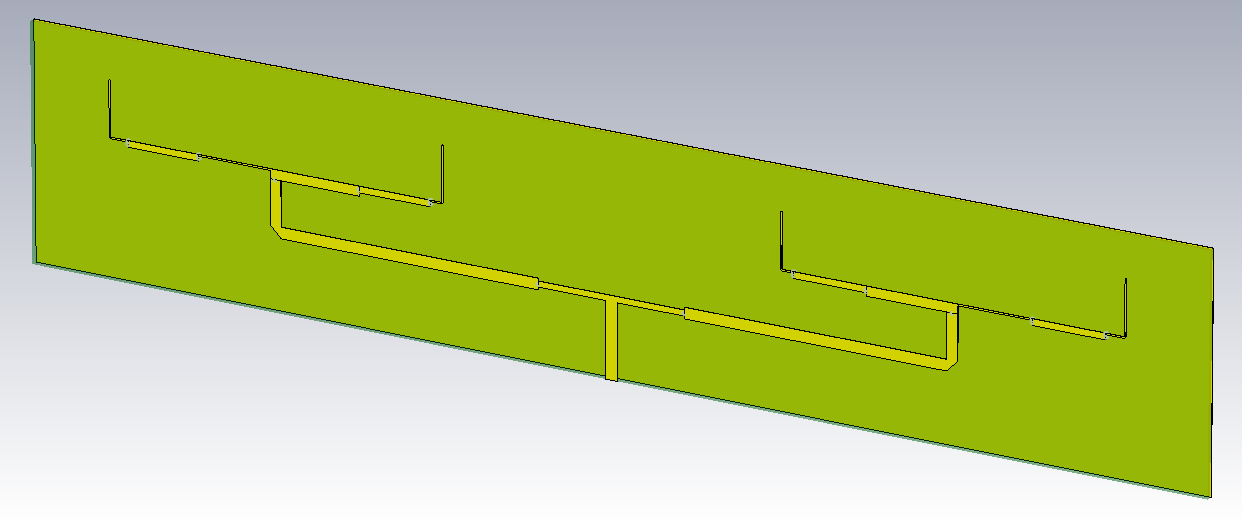
\includegraphics[scale=0.45]{layout.png}
\caption{How our BFN looks like}
\label{layout}
\end{figure}

\subsection{Simulation with \textit{Microwave Studio}}

Unfortunately, if till this point the simulations seemed to be very encouraging, we realized that when trying to transfer the design on \textit{CST Microwave Studio} they were not so good: the resonance was not as precise as we'd have expected and neither was the tapering. Furthermore, if using the optimizer turned out to be a very useful tool when using \textit{Design Studio}, things are not so easy in \textit{Microwave Studio}, where the high density of the mesh needed in order to obtain reliable results makes the simulation time very long. Due to these reasons we began from scratch, trying to build up the single components of the BFN separately. As previously described the power splitters seem to work on their own, giving the correct power ratio and phasing, but even in this case we were not able to put them together obtaining immediately a satisfactory result, nor we managed to optimize the results on the base of what previously obtained as well as we did in \textit{Design Studio}. The reasons are multiple: long simulation time (as already mentioned) if the mesh is dense and low reliability if, with the aim of reducing the simulation time to allow for optimization, one uses a larger meshgrid, very high precision of the optimizer, which specifies a lot of digits (which has no sense if one thinks about the specifications one should give the producer in order to print the antenna). Furthermore: every curve introduces a non ideality and even the simple lines are not easy to tune all together to the correct impedance value. Simulations were carried out both with discrete face ports (whose reference impedance can be specified by the user) and with waveguide ports, with which we were finally able to obtain an acceptable result, even if not perfect as one would like.
\par\medskip
\noindent

In the following figures: the globally best result we obtained in \textit{Microwave Studio}, resonating at the right frequency even if the shape of the curve is not exceptional and with acceptable tapering:

\begin{figure}[H]
\centering
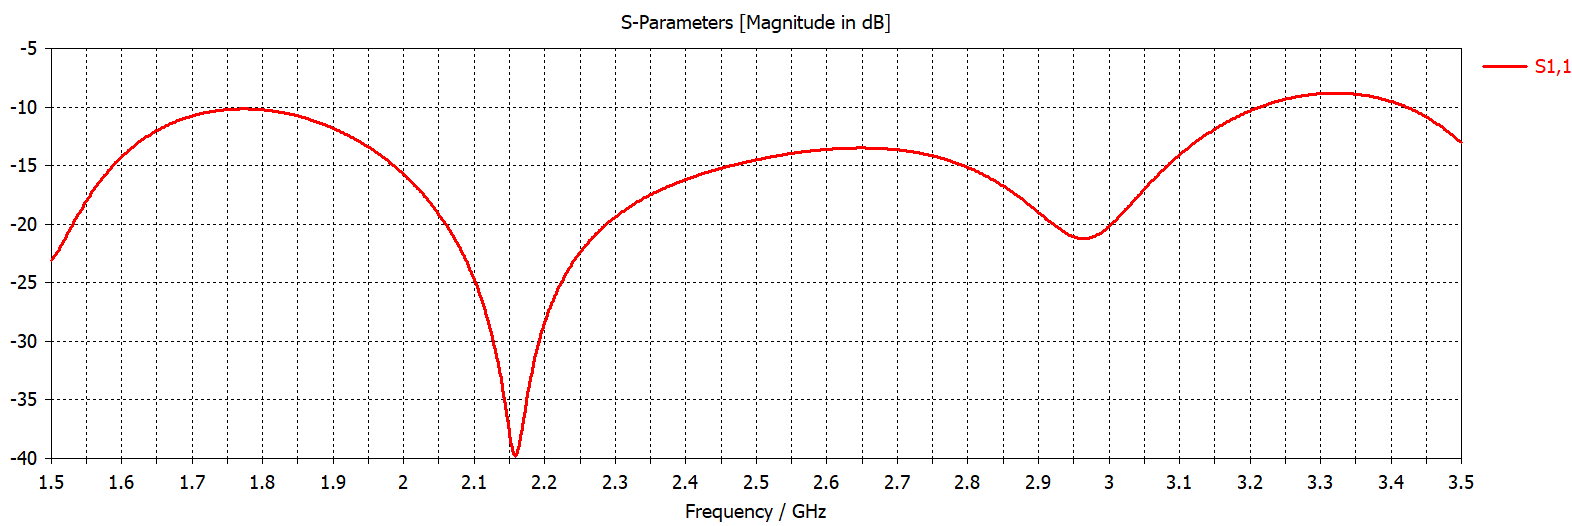
\includegraphics[scale=0.35]{11.png}
\caption{S\textsubscript{11} parameter, not resonating correctly}
\label{a}
\end{figure}

\begin{figure}[H]
\centering
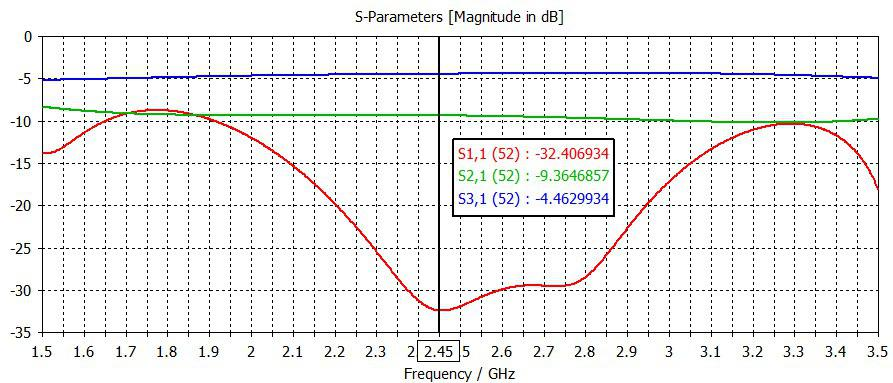
\includegraphics[scale=0.35]{cacca.jpg}
\caption{amplitude of the important parameters}
\label{a}
\end{figure}

\begin{figure}[H]
\centering
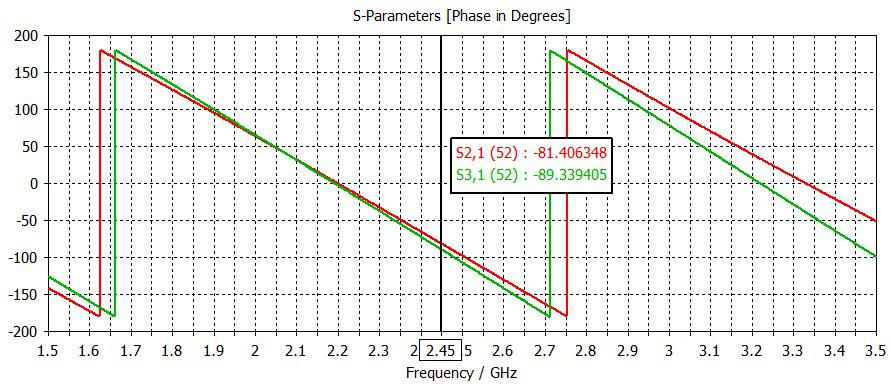
\includegraphics[scale=0.35]{cacca1.jpg}
\caption{phase of the important parameters}
\label{b}
\end{figure}


\par\medskip
\noindent
It is important to notice that S\textsubscript{21} coincides with S\textsubscript{51}, while S\textsubscript{31} coincides with S\textsubscript{41}. This was predictable, but it is also due to the fact that we imposed as a boundary condition a simmetry plane (xy) for the magnetic field, since the simmetry of the system allows for it: the field lines are closed around the microstrip at the input port and the tangent camponent is null in the xy plane.

\begin{figure}[H]
\centering
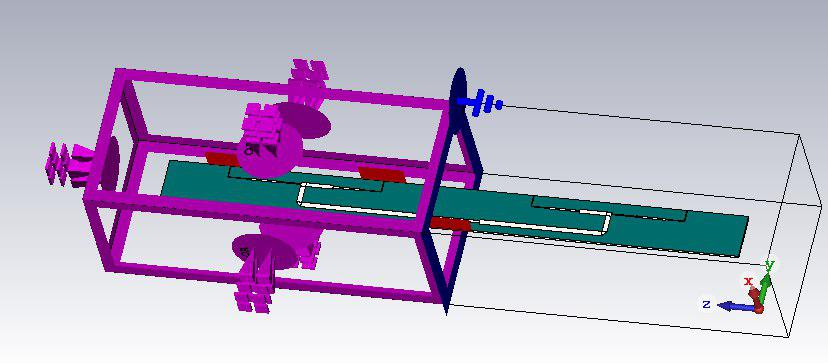
\includegraphics[scale=0.35]{sonostanco.jpg}
\caption{simmetry plane adopted}
\label{c}
\end{figure}

\par\medskip
\noindent
We also tried to simulate the behavior of the BFN when attached to the patches, but, since the tapering was not the good one we had hoped for, the SLL wasn't completely tuned on the -20 dB level either. Good notes are the fact that the radiated field happened to be broadside, meaning that the phasing, at least, was correct, and that the resonance frequency, even if not perfect, happened to be more precise in this case. A more specific and precise analysis of the obtained AF will be discussed in the last part.